

\begin{frame}[fragile]{Hello, \LaTeX!}

  \begin{columns}
    \begin{column}{.7\linewidth}
      \begin{itemize}
        \item Create \mintinline{text}|hello.tex| file with following content.
              \inputminted{latex}{./minted/hello.tex}
        \item Compile it
              \begin{itemize}
                \item Click the build button in your \LaTeX~editor/IDE
                \item OR using command line: \bashinline|latexmk -pdf hello|
              \end{itemize}
        \item Open \mintinline{text}|hello.pdf| to preview the result
      \end{itemize}
    \end{column}

  \begin{column}{.3\linewidth}
      \begin{figure}
        \centering
        %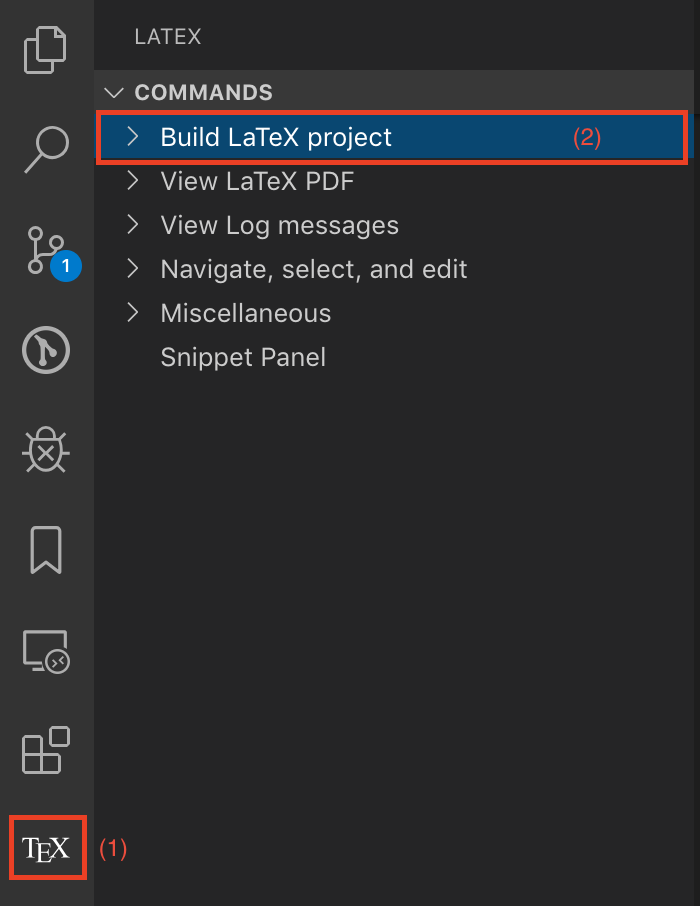
\includegraphics[width=\linewidth]{./figs/vscode-compile-project.png}
        \caption{Compile \LaTeX~Project in VSCode}
      \end{figure}
    \end{column}
  \end{columns}
\end{frame}

\begin{frame}[fragile]{Example of A Complex Document}
  \begin{itemize}
    \item Download the source code from \url{https://github.com/xu-cheng/latex-tutorial/archive/master.zip}
    \item The example document is located in the \mintinline{text}|example| folder. It contains:
          \begin{itemize}
            \item \mintinline{text}|main.tex| The main tex source
            \item \mintinline{text}|preamble.tex| A subfile to store format definitions
            \item \mintinline{text}|tikz-example.tex| A figure drawn using tikz
            \item \mintinline{text}|ref.bib| A database of references
          \end{itemize}
    \item Use \bashinline|latexmk -pdf main| to compile the document
    \item Access the same example in Overleaf: \url{https://www.overleaf.com/read/qsthqbjphhrz}
  \end{itemize}
\end{frame}

% \begin{noindent}
\begin{frame}[fragile]{Comment, Command and Environment}
  \begin{itemize}
    \item \latexinline|%| starts a comment. e.g.~\latexinline|% this is hello.tex|
    \item \latexinline|\| starts a command.
          \begin{latexcode}
            \command % a command
            \command{} % also a command
            \command{arg} % a command with an argument
            \command{arg1}{arg2} % a command with multiple arguments
            \command[opt arg]{arg} % [] is for optional argument
          \end{latexcode}
    \item \latexinline|\begin{} ... \end{}| denotes an environment
          \begin{latexcode}
            \begin{envname}
              inside the environment
            \end{envname}
            % LaTeX environment can take arguments
            \begin{envname}{arg} \end{envname}
            \begin{envname}[opt arg]{arg} \end{envname}
          \end{latexcode}
  \end{itemize}
\end{frame}
% \end{noindent}

\begin{frame}[fragile]{Source File Structure}
  \begin{itemize}
    \item A document starts with \latexinline|\documentclass{...}| command to specify the template
    \item Common templates include:
          \setlength{\multicolsep}{0pt}
          \setlength{\columnsep}{0pt}
          \begin{multicols}{3}
            \begin{itemize}
              \item \texttt{article}
              \item \texttt{book}
              \item \texttt{report}
              \item \texttt{letter}
              \item \texttt{beamer} \textsmaller{(slides)}
              \item \texttt{standalone} \textsmaller{(graphics)}
              \item \texttt{acmart} \textsmaller{(ACM~template)}
              \item \texttt{IEEEtrans} \textsmaller{(IEEE~template)}
              \item[]
            \end{itemize}
          \end{multicols}
    \item Template class can accept options, e.g.~\latexinline|\documentclass[a4paper,10pt]{article}|
  \end{itemize}

  \begin{block}{Class Options for \texttt{article}, \texttt{report}, \texttt{book}, \texttt{letter}}
    \begin{description}[\scriptsize\texttt{titlepage}, \texttt{notitlepage}]
      \scriptsize
      \item[\normalfont\texttt{10pt}, \texttt{11pt}, \texttt{12pt}] \quad Set font size.
      \item[\normalfont\texttt{a4paper}, \texttt{letterpaper}, \ldots] \quad Defines
            the paper size.
      \item[\normalfont\texttt{fleqn}] \quad Typesets displayed formulae left-aligned
            instead of centred.
      \item[\normalfont\texttt{leqno}] \quad Places the numbering of formulae on the
            left hand side instead of the right.
      \item[\normalfont\texttt{titlepage}, \texttt{notitlepage}] \quad Specifies whether a new page should be started after the document title or not.
      \item[\normalfont\texttt{onecolumn}, \texttt{twocolumn}] \quad Typeset the document in one column or two columns.
      \item[\normalfont\texttt{twoside, oneside}] \quad Specifies whether double or single sided output should be generated.
      \item[\normalfont\texttt{landscape}] \quad Changes the layout of the document to print in landscape mode.
      \item[\normalfont\texttt{openright, openany}] \quad Makes chapters begin either only on right hand pages or on the next page available.
    \end{description}
  \end{block}
\end{frame}



\begin{frame}[fragile]{Hello, \LaTeX!}

  \begin{columns}
    \begin{column}{.7\linewidth}
      \begin{itemize}
        \item Create \mintinline{text}|hello.tex| file with following content.
              \inputminted{latex}{./minted/hello.tex}
        \item Compile it
              \begin{itemize}
                \item Click the build button in your \LaTeX~editor/IDE
                \item OR using command line: \bashinline|latexmk -pdf hello|
              \end{itemize}
        \item Open \mintinline{text}|hello.pdf| to preview the result
      \end{itemize}
    \end{column}

  \begin{column}{.3\linewidth}
      \begin{figure}
        \centering
        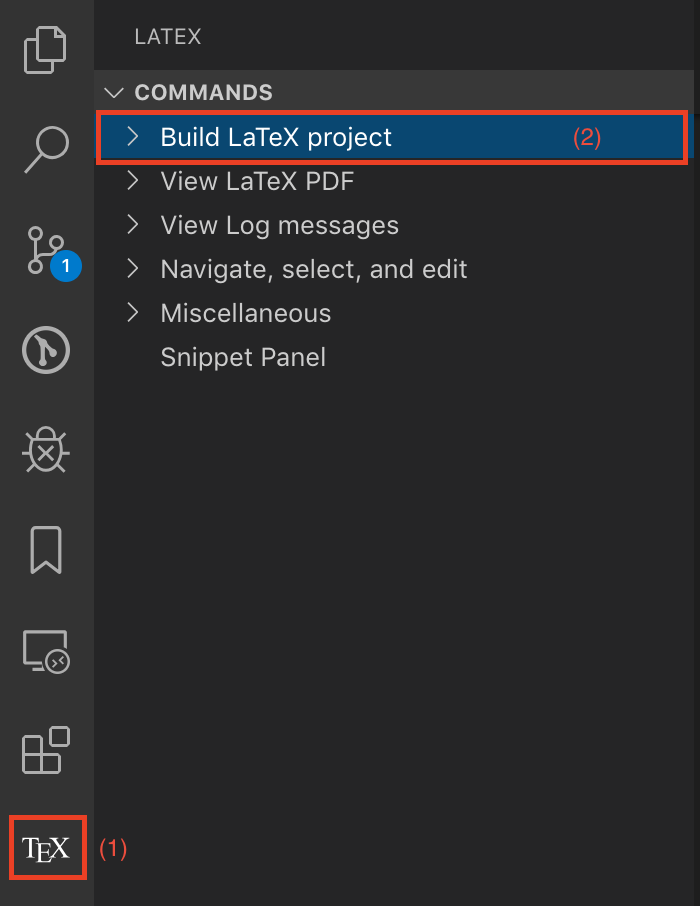
\includegraphics[width=\linewidth]{./figs/vscode-compile-project.png}
        \caption{Compile \LaTeX~Project in VSCode}
      \end{figure}
    \end{column}
  \end{columns}
\end{frame}

\begin{frame}[fragile]{Example of A Complex Document}
  \begin{itemize}
    \item Download the source code from \url{https://github.com/xu-cheng/latex-tutorial/archive/master.zip}
    \item The example document is located in the \mintinline{text}|example| folder. It contains:
          \begin{itemize}
            \item \mintinline{text}|main.tex| The main tex source
            \item \mintinline{text}|preamble.tex| A subfile to store format definitions
            \item \mintinline{text}|tikz-example.tex| A figure drawn using tikz
            \item \mintinline{text}|ref.bib| A database of references
          \end{itemize}
    \item Use \bashinline|latexmk -pdf main| to compile the document
    \item Access the same example in Overleaf: \url{https://www.overleaf.com/read/qsthqbjphhrz}
  \end{itemize}
\end{frame}

% \begin{noindent}
\begin{frame}[fragile]{Comment, Command and Environment}
  \begin{itemize}
    \item \latexinline|%| starts a comment. e.g.~\latexinline|% this is hello.tex|
    \item \latexinline|\| starts a command.
          \begin{latexcode}
            \command % a command
            \command{} % also a command
            \command{arg} % a command with an argument
            \command{arg1}{arg2} % a command with multiple arguments
            \command[opt arg]{arg} % [] is for optional argument
          \end{latexcode}
    \item \latexinline|\begin{} ... \end{}| denotes an environment
          \begin{latexcode}
            \begin{envname}
              inside the environment
            \end{envname}
            % LaTeX environment can take arguments
            \begin{envname}{arg} \end{envname}
            \begin{envname}[opt arg]{arg} \end{envname}
          \end{latexcode}
  \end{itemize}
\end{frame}
% \end{noindent}

\begin{frame}[fragile]{Source File Structure}
  \begin{itemize}
    \item A document starts with \latexinline|\documentclass{...}| command to specify the template
    \item Common templates include:
          \setlength{\multicolsep}{0pt}
          \setlength{\columnsep}{0pt}
          \begin{multicols}{3}
            \begin{itemize}
              \item \texttt{article}
              \item \texttt{book}
              \item \texttt{report}
              \item \texttt{letter}
              \item \texttt{beamer} \textsmaller{(slides)}
              \item \texttt{standalone} \textsmaller{(graphics)}
              \item \texttt{acmart} \textsmaller{(ACM~template)}
              \item \texttt{IEEEtrans} \textsmaller{(IEEE~template)}
              \item[]
            \end{itemize}
          \end{multicols}
    \item Template class can accept options, e.g.~\latexinline|\documentclass[a4paper,10pt]{article}|
  \end{itemize}

  \begin{block}{Class Options for \texttt{article}, \texttt{report}, \texttt{book}, \texttt{letter}}
    \begin{description}[\scriptsize\texttt{titlepage}, \texttt{notitlepage}]
      \scriptsize
      \item[\normalfont\texttt{10pt}, \texttt{11pt}, \texttt{12pt}] \quad Set font size.
      \item[\normalfont\texttt{a4paper}, \texttt{letterpaper}, \ldots] \quad Defines
            the paper size.
      \item[\normalfont\texttt{fleqn}] \quad Typesets displayed formulae left-aligned
            instead of centred.
      \item[\normalfont\texttt{leqno}] \quad Places the numbering of formulae on the
            left hand side instead of the right.
      \item[\normalfont\texttt{titlepage}, \texttt{notitlepage}] \quad Specifies whether a new page should be started after the document title or not.
      \item[\normalfont\texttt{onecolumn}, \texttt{twocolumn}] \quad Typeset the document in one column or two columns.
      \item[\normalfont\texttt{twoside, oneside}] \quad Specifies whether double or single sided output should be generated.
      \item[\normalfont\texttt{landscape}] \quad Changes the layout of the document to print in landscape mode.
      \item[\normalfont\texttt{openright, openany}] \quad Makes chapters begin either only on right hand pages or on the next page available.
    \end{description}
  \end{block}
\end{frame}


